\documentclass{beamer}
\usepackage{beamerthemesplit}
\usepackage{wrapfig}
\usetheme{SPbGU}
\usepackage{pdfpages}
\usepackage{amsmath}
\usepackage{cmap} 
\usepackage[T2A]{fontenc} 
\usepackage[utf8]{inputenc}
\usepackage[english,russian]{babel}
\usepackage{indentfirst}
\usepackage{amsmath}
\usepackage{tikz}
\usepackage{multirow}
\usepackage[noend]{algpseudocode}
\usepackage{algorithm}
\usepackage{algorithmicx}
\usepackage{pgf}
\usepackage{tikz}
% \usepackage[latin1]{inputenc}
\usetikzlibrary{shapes,arrows,automata}
\usepackage{fancyvrb}
\newtheorem{rutheorem}{Теорема}
\newtheorem{ruproof}{Доказательство}
\newtheorem{rudefinition}{Определение}
\newtheorem{rulemma}{Лемма}
\beamertemplatenavigationsymbolsempty

\title[]{Поддержка произвольных конечных автоматов в алгоритме синтаксического анализа регулярной аппроксимации кода на встроенных языках}
\subtitle[]{YaccConstructor}
% То, что в квадратных скобках, отображается в левом нижнем углу. 
\institute[]{
Лаборатория языковых инструментов JetBrains}

% То, что в квадратных скобках, отображается в левом нижнем углу.
\author[И. Шугаепов]{И. Шугаепов \\ Руководитель: Е. Вербицкая}

\date{21 декабря 2015}

\definecolor{orange}{RGB}{179,36,31}

\begin{document}
{
\begin{frame}[fragile]
  \begin{tabular}{p{2.5cm} p{5.5cm} p{2cm}}
   \begin{center}
      
\includegraphics[width=2.5cm]{pictures/JBLogoWhite.png}
    \end{center}
    &
    \begin{center}
      
\includegraphics[width=1cm]{pictures/au.png}
    \end{center}
    &
    \begin{center}
      
\includegraphics[width=1cm]{pictures/YC_big.jpg}
    \end{center} 
  \end{tabular}
  \titlepage
\end{frame}
}
            

\begin{frame}[fragile]
  \transwipe[direction=90]
  \frametitle{Сфера применимости алгоритма}
\begin{tabular}{p{4.5cm} p{8cm}}
Встроенный код
&
\begin{minipage}[t]{5cm}

\begin{Verbatim}[commandchars=\\\{\}]
\textcolor{blue}{string} res = \textcolor{orange}{""};
\textcolor{blue}{for}(i = 0; i < l; i++)
    res = \textcolor{orange}{"()"} + res;
\fbox{\textcolor{blue}{use}(res);}

\end{Verbatim}
\end{minipage}

\\ 
Возможные значения
&
\begin{minipage}[t]{2.5cm}
\begin{Verbatim}[commandchars=\\\{\}]
\{\textcolor{orange}{""}, \textcolor{orange}{"()"},  \textcolor{orange}{"()()"}, ..., \textcolor{orange}{"()"}^l\}
\end{Verbatim}
\end{minipage}

\\
Аппроксимация
&
\begin{minipage}[t]{4cm}
  \begin{Verbatim}[commandchars=\\\{\}]
(\textcolor{orange}{"()"})*
  \end{Verbatim} 
\end{minipage}

\\
Соответствующий КА
&
\begin{minipage}[t]{3cm}                        
\raisebox{-\height}{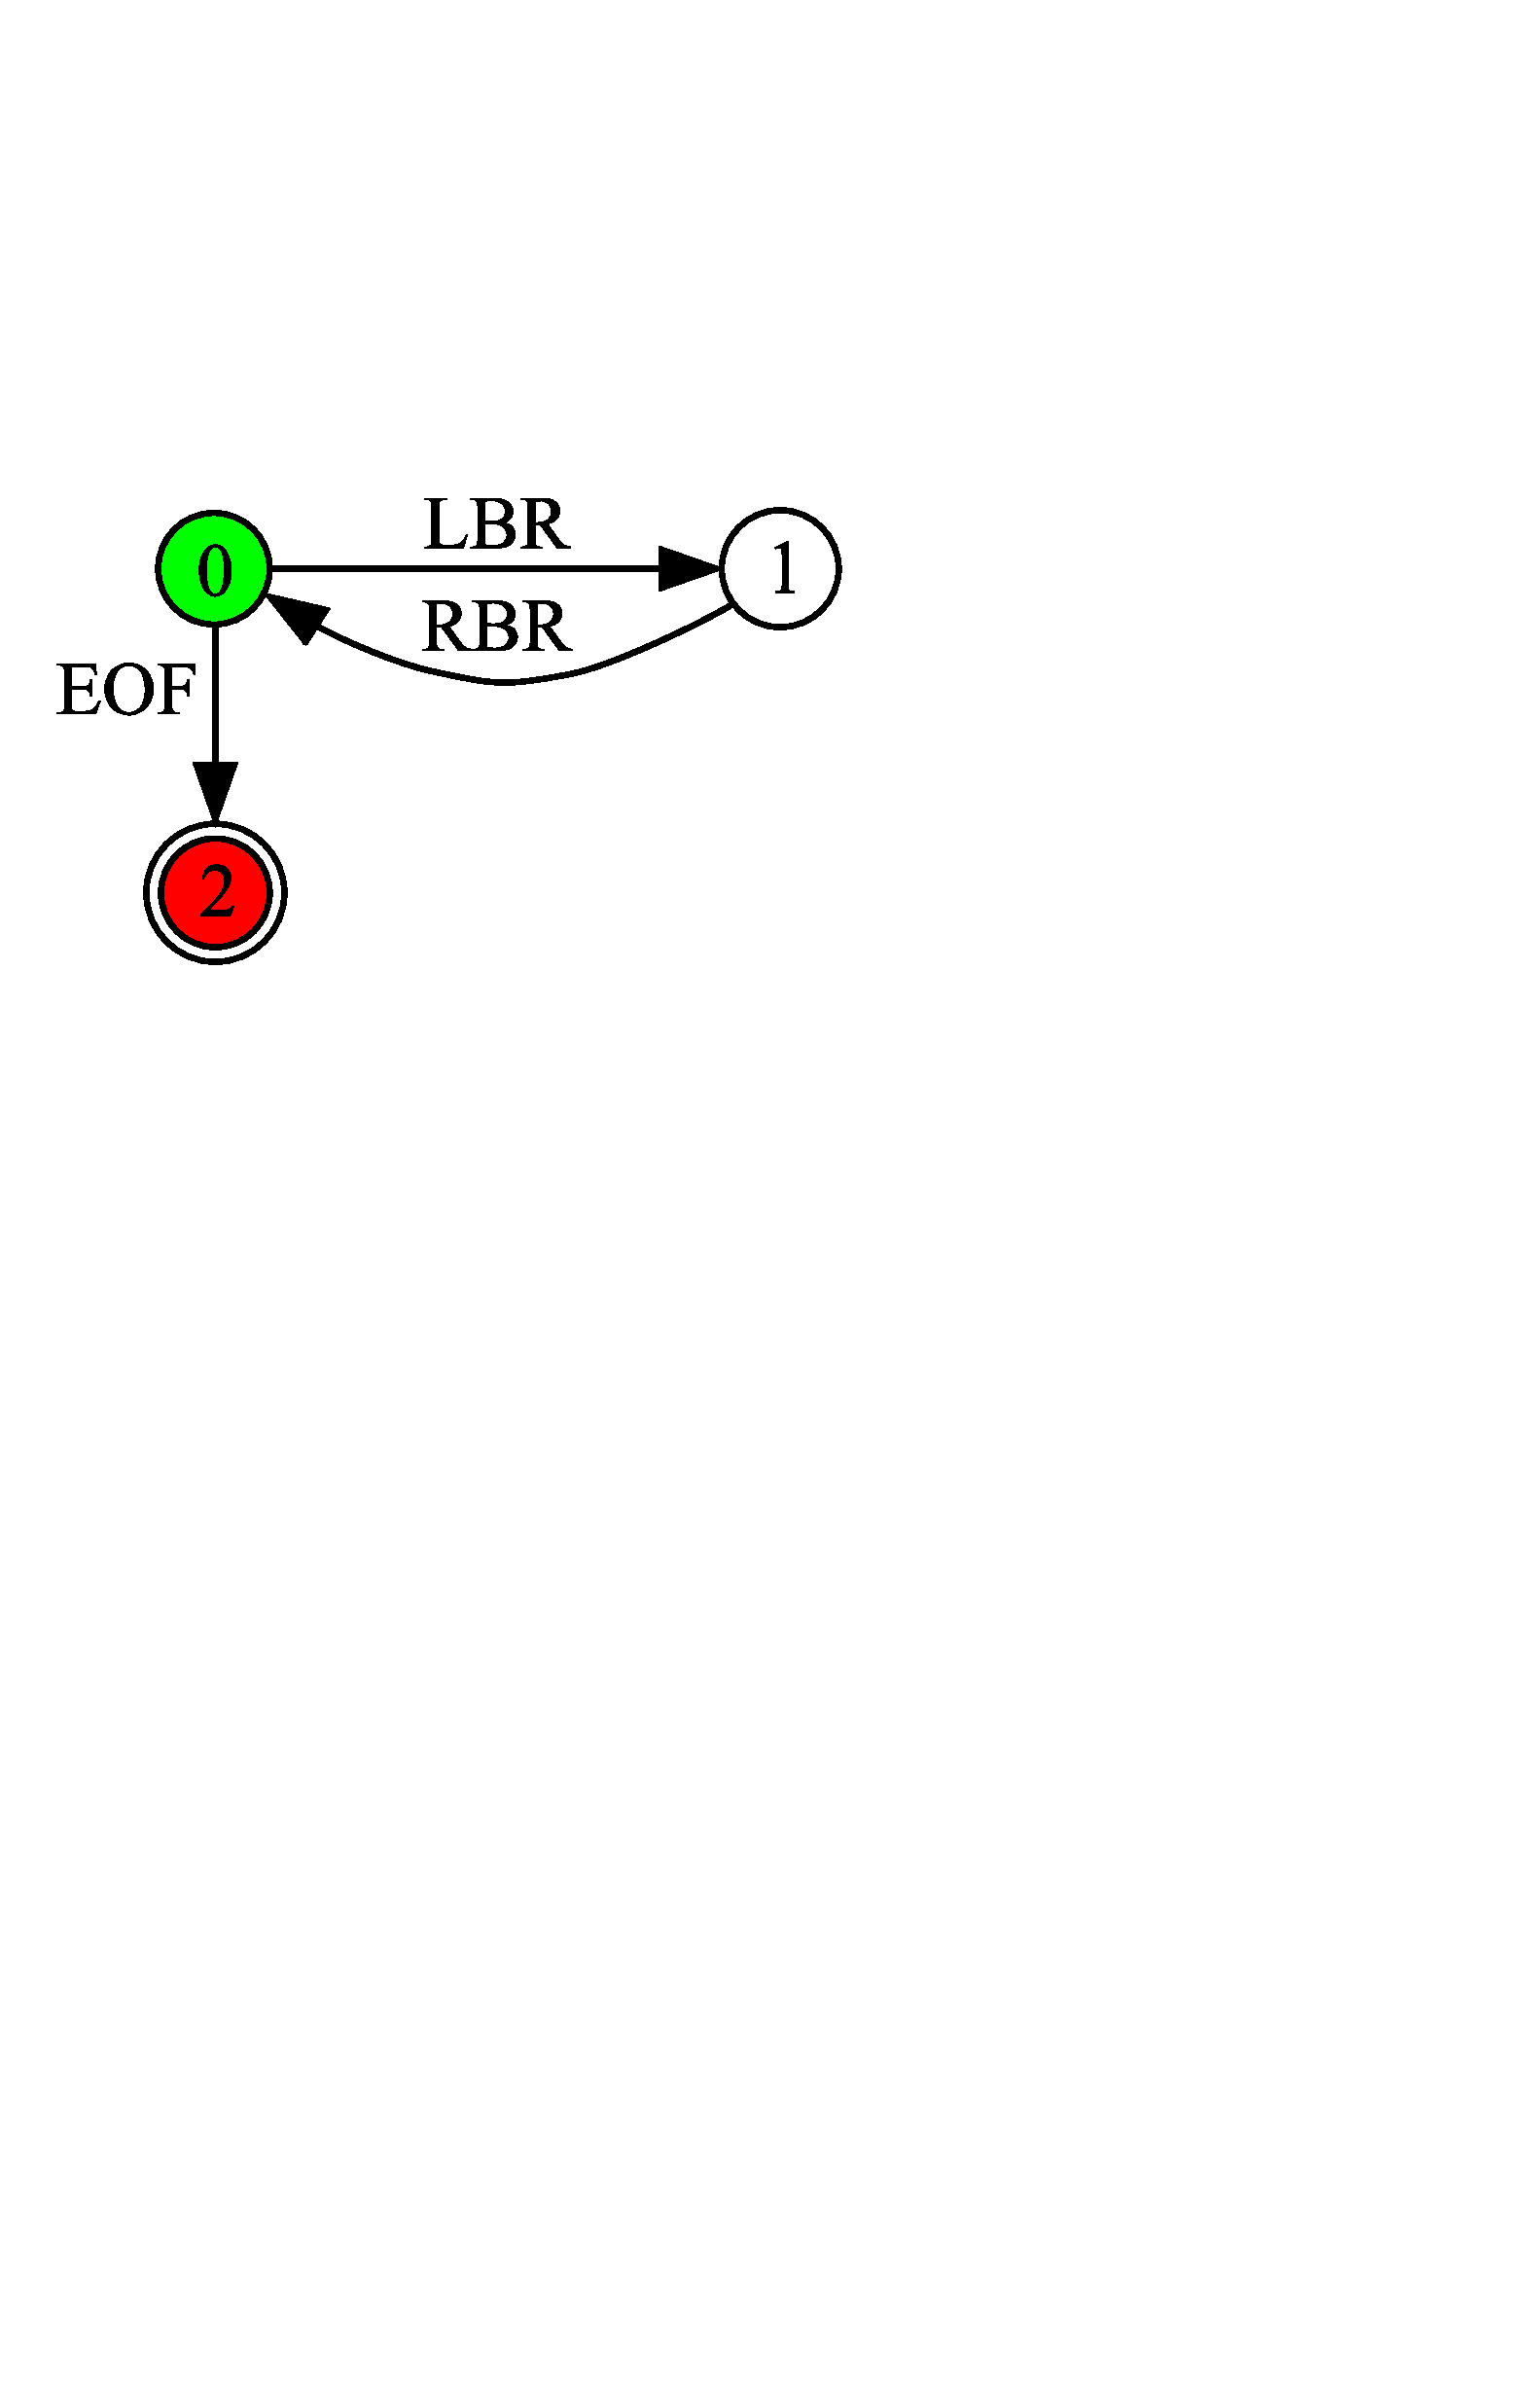
\includegraphics[width=3cm]{pictures/in31}}
\end{minipage}


\end{tabular}

\end{frame}

\begin{frame}
  \transwipe[direction=90]
  \frametitle{Алгоритм}
  \begin{itemize}
    \item \textbf{Вход:}
        КС-грамматика $ G $ и конечный автомат над алфавитом терминалов из $ G $
    \item \textbf{Выход:}
        конечное представление множества деревьев,
        соответствующих всем корректным цепочкам, принимаемым
        входным автоматом
  \end{itemize}
\end{frame}


\begin{frame}
  \transwipe[direction=90]
  \frametitle{Цели и задачи}
  \textbf{Целью} работы было снятие ограничений на входную структуру данных (входной автомат). То есть:\\
  Детерминированный автомат без $\epsilon$-переходов $\Rightarrow$ произвольный конечный автомат. \\
  \textbf{Задачи:}
  \begin{itemize}
        \item Поддержать множественные исходящие ребра с одинаковыми метками
        \item Поддержать множественные начальные вершины
        \item Поддержать множественные конечные вершины
        \item Поддержка $\epsilon$ переходов
  \end{itemize}
\end{frame}

\begin{frame}
  \transwipe[direction=90]
  \frametitle{Теория}
  \begin{itemize}
    \item \text{Left-to-right Rightmost derivation parser (LR)}
    \item \text{Generalized LR (Tomita)}
    \item \text{Right Nulled Generalized LR}
  \end{itemize}
\end{frame}

\begin{frame}
\transwipe[direction=90]
\frametitle{Пример 1}
\begin{tabular}{p{5.5cm} p{5.5cm}}
\begin{center}
Входной автомат: \\
$ $\\
\begin{tikzpicture}[->,>=stealth',shorten >=1pt,auto,node distance=2cm,
                    semithick]
  \tikzstyle{every state}=[fill=none,draw=black,text=black, scale=0.6]

  \node[state] (A)                    {$0$};
  \node[state]         (B) [right of=A] {$1$};
  \node[state]         (C) [below right of=B] {$2$};
  \node[state]         (D) [above right of=C] {$3$};
  \node[state]         (E) [above left of=D] {$4$};
  \node[state]         (F) [right of=D] {$5$};
  \node[state,accepting]         (G) [right of=F] {$6$};

  \path (A) edge              node {$(_1$} (B)
        (B) edge [loop above] node {$(_2$} (B)
            edge              node {$\epsilon$} (C)
        (C) edge              node {$\epsilon$} (D)
        (D) edge              node {$\epsilon$} (E)
        (E) edge              node {$\epsilon$} (B)
        (D) edge              node {$)_3$} (F)
        (F) edge              node {eof} (G)
            edge [loop below] node {$)_4$} (F);
\end{tikzpicture}
\end{center}
&
\begin{center}
    \text{SPPF:}\\
    $ $\\
    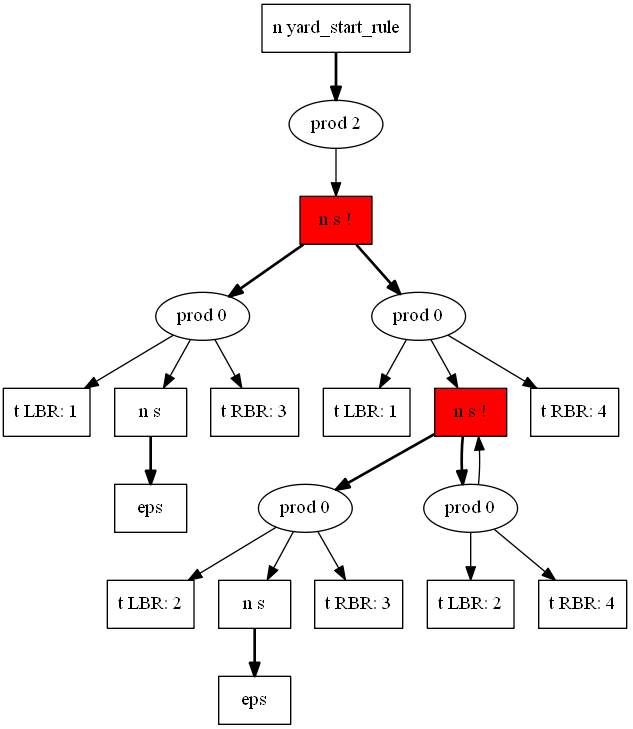
\includegraphics[scale=0.68]{pictures/sppf.png}
\end{center}
\end{tabular}
\end{frame}

\begin{frame}
\transwipe[direction=90]
\frametitle{Пример 2}
\begin{tabular}{p{5.5cm} p{5.5cm}}
\begin{center}
Входной автомат: \\
$ $\\
\begin{tikzpicture}[->,>=stealth',shorten >=1pt,auto,node distance=2.5cm,
                    semithick]
  \tikzstyle{every state}=[fill=none,draw=black,text=black, scale=0.5]

  \node[initial,state] (A)                    {$0$};
  \node[state]         (B) [right of=A] {$1$};
  \node[state,accepting]         (C) [above right of=B] {$5$};
  \node[initial,state]         (D) [below right of=B] {$2$};
  \node[state]         (E) [below right of=D] {$3$};
  \node[state,accepting]         (F) [below right of=E] {$4$};

  \path (A) edge              node {$num_1$} (B)
        (B) edge              node {$+_2$} (D)
            edge              node {$eof$} (C)
        (D) edge              node {$num_3$} (E)
        (E) edge              node {$eof$} (F);
\end{tikzpicture}
\end{center}
&
\begin{center}
    \text{SPPF:}\\
    $ $\\
    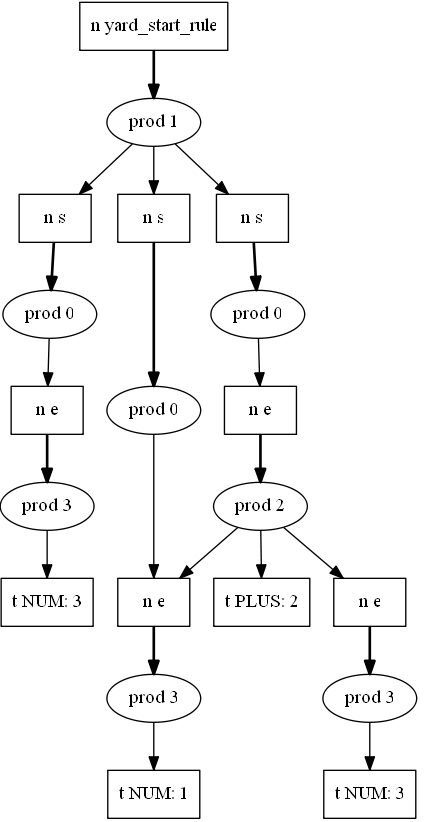
\includegraphics[scale=0.6]{pictures/sppf2.png}
\end{center}
\end{tabular}
\end{frame}

\begin{frame}
\transwipe[direction=90]
\frametitle{Результаты}
\begin{itemize}
\item Реализована поддержка:
\begin{itemize}
  \item Множественных исходящих ребра с одинаковыми метками
  \item Множественных начальных вершины
  \item Множественных конечных вершины
\end{itemize}
\item Частично реализовано:
\begin{itemize}
  \item Поддержка $\epsilon$ переходов
\end{itemize}
\end{itemize}
Исходный код YaccConstructor: \url{https://github.com/YaccConstructor/YaccConstructor} \\
    Ветка  \text{iss103 eps}
\end{frame}

\end{document}
